\chapter{Implementation}\label{chp:implementation}

\section{Introduction}

An obstruction detector and a vanishing point detector are the two attempted implementations presented in this report. The obstruction detector uses stereo vision to perceive depth and distance to possible objects in the path of the robot. The vanishing point detector attempts to find a single vanishing point by detecting lines in the environment before selecting a vanishing point based on line intersections. 

\section{Vanishing Point Detection}

\subsection{Overview}

The goal of the vanishing point detector is to provide a setpoint for the robot to steer towards. In other words, steering towards a vanishing point is a good way to reach the end of a hallway or corridor. This was considered to be a good starting point, and possible expantions could be added later. Choosing a method as a basis for a vanishing point detector was not easy. The selected method should be simple, suitable for \gls{opencv} and not go too far beyond the prior knowledge of the author. Another important factor was that spending too much time on this implementation would come at the expense of the obstruction detector. A vanishing point detector method by D. Gerogiannis et. al. \cite{gerogiannisvp} showed promise as it was based on line detection, which has good support in OpenCV. The method in \cite{gerogiannisvp} appears to be suitable for structured environments with many straight lines, such as hallways, streets and corridors. The steps in the detection procedure are:

\begin{enumerate}
	\item Detect edges in the image, e.g. by using Canny edge detection.
	\item Detect line segments that may be used as vanishing lines based on edges found in step 1. Could be done with the Hough line transform.
	\item Filter the detected lines. This is done by modelling new lines by using the major axis of ellipses with very high eccentricity. The ellipses are generated by a split-and-merge algorithm. In short, it will merge similar line segments by assuming that their end points are collinear.
	\item Find line intersection points based on the new filtered lines. Each point is stored and assigned a weight.
	\item Find the vanishing point among the line intersections based on a voting scheme. 
\end{enumerate}

\subsection{Line Detection}

Line detection comprise step 1 and 2 from the list above. OpenCV comes with an implementation of the Canny edge detector ready for use. The detector returns a binary image of the detected edges. Edges are detected by convolving the input image with two kernels $G_x$ and $G_y$. The convolutions will indicate change gradients in the $x$ and $y$ directions which in turn will give the direction of a potential edge. Finally, the detector rejects or accepts potential edges based on two gradient thresholds. Gradients below the lower threshold are rejected, edges above the upper threshold are accepted, and edges between the thresholds are only accepted if their neighbouring gradients are above the upper threshold\cite{cannyedge}. 

\begin{wrapfigure}{r}{0.55\textwidth}
	\vspace{-10pt} % Remove exessive whitespace
	\centering
	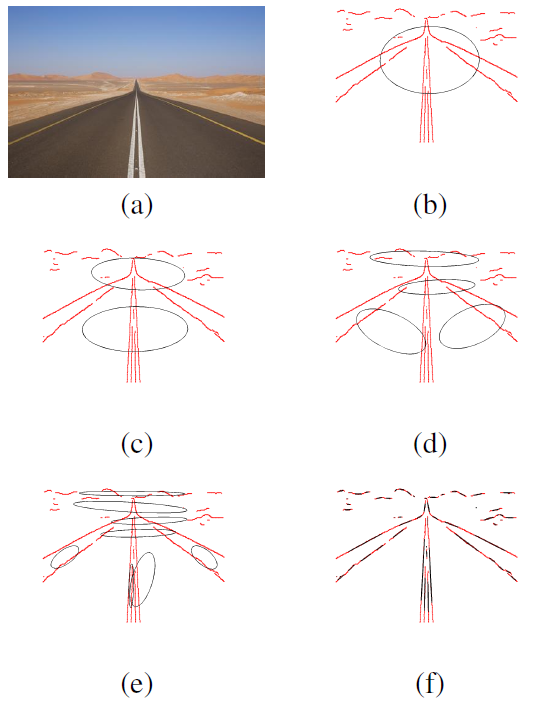
\includegraphics[width=0.6\textwidth]{GerogiannisLines}
	\caption{\label{fig:GerogiannisLines}Gerogiannis concept of representing lines by eccentric ellipses. This image is taken directly from \cite{gerogiannisvp}.}
	\vspace{-60pt} % Remove exessive whitespace
\end{wrapfigure}

At this point, we only have a simple binary image where edges are represented as white pixels on a black background. The next step is to interpret these edges as lines. Line detection is performed by using the probabilistic Hough line transform. This is an already implemented function, which takes in the edge image from the previous step, and return a set of point pairs representing line segments. The benefit of using the probabilistic detector is that it can perceive an edge with a discontinuity as a singe line. 

\subsection{Line Filtering}

Line filtering is performed by splitting and merging ellipses until their major axis represents a set of approximations to collinear points. The points is the set of points that define the previously detected line segments. This algorithm is called \gls{dsam}, and it is explained in another paper by D. Gerogiannis \cite{gerogiannisshape}. Line segments returned from the probabilistic Hough transform will often overlap or be very close to each other. The purpose of this step is to get a cleaner representation of the contours in the environment.

Figure \ref{fig:GerogiannisLines}, taken from \cite{gerogiannisvp}, illustrates the steps in the \gls{dsam} algorithm.

\subsection{Vanishing Point Detection}

\begin{wrapfigure}{r}{0.35\textwidth}
	\vspace{-10pt} % Remove exessive whitespace
	\centering
	\includegraphics[width=0.36\textwidth]{getVp}
	\caption{\label{fig:getVp}Two steps in "getVanishingPoint()".}
	\vspace{-60pt} % Remove exessive whitespace
\end{wrapfigure}


When the detected lines have been filtered and stored, they will be passed to the vanishing point detector in the function "getVanishingPoint(lines)". This function will perform two steps (figure \ref{alg:getVp}):

\begin{enumerate}
	\item Find, store and assign weights to the points where the lines intersect. Lines that are either too vertical or too horizintal will not be included in the calculations. Intersectionpoints outside the image frame are rejected.
	\item Find the vanishing point based on the valid weighted intersection points. This is done by a voting scheme described in \cite{gerogiannisvp}, and illustrated as a flowchart in figure \ref{fig:findVp}. 
\end{enumerate}

\begin{figure}
	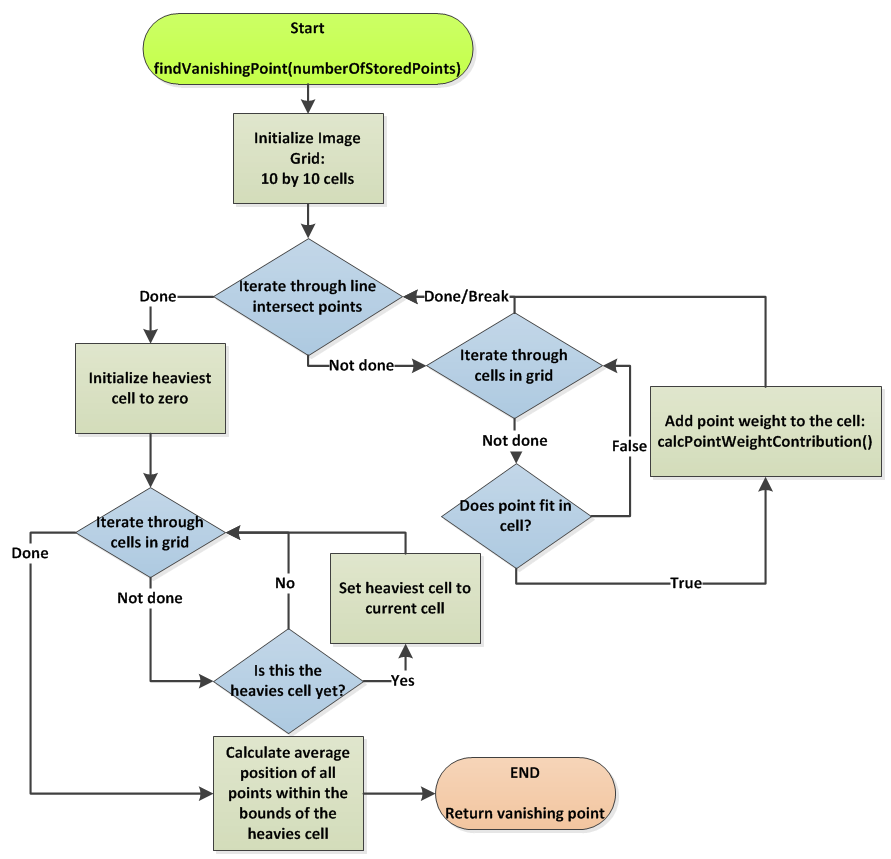
\includegraphics[scale=0.5]{findVp}
	\caption{Sequence diagram illustrating program execution when the user activates camera feed and VP detection.}
	\label{fig:findVp}
\end{figure}

\subsection{Vanishing Point Detector Application}

\paragraph{Program Structure}

The vanishing point detector was implemented as a QWidget Application in the Qt Creator IDE. The code excerpt shown in algorithm \ref{alg:edgelines} contains the most important image processing steps. A main thread, which may be called the GUI thread, handles all user related input and output. All image processing is done in the class "ImageProcessing" which inherits from QThread. This means that "ImageProcessing" controls a protected function "run()" which contains the threaded code and image processing steps. Figure \ref{fig:VpAppSequence} is a sequence diagram that shows the different classes and threads interact. The ellipse filter step is ommitted in the illustration; if it had been included, it would be called between "hough->detect()" and "getVanishingPoint()".

\begin{algorithm}[h]
	\caption{Vanishing point detector loop. Several lines of code are omitted in this example to make the processing more clear.}
	\label{alg:edgelines}
	\begin{verbatim}
	while(){
		capture.read(cameraImg);
		cvtColor(cameraImg,grayImg,CV_RGB2GRAY);
		blur( grayImg, blurredImg, Size(3,3) );
		Canny(blurredImg, edgesImg, lowerThresh, upperThresh, 3);
		gpu_edgesImg.upload(edgesImg);
		lines = detectHoughLines(gpu_edgesImg);   
		newLines = mLineEllipseFilter.filterLines(lines,originalImage);
		Point vanishingPoint = vpDetector.getVp(newLines,cameraImg);     
	}
	\end{verbatim}
\end{algorithm}

\begin{landscape}
	\begin{figure}
		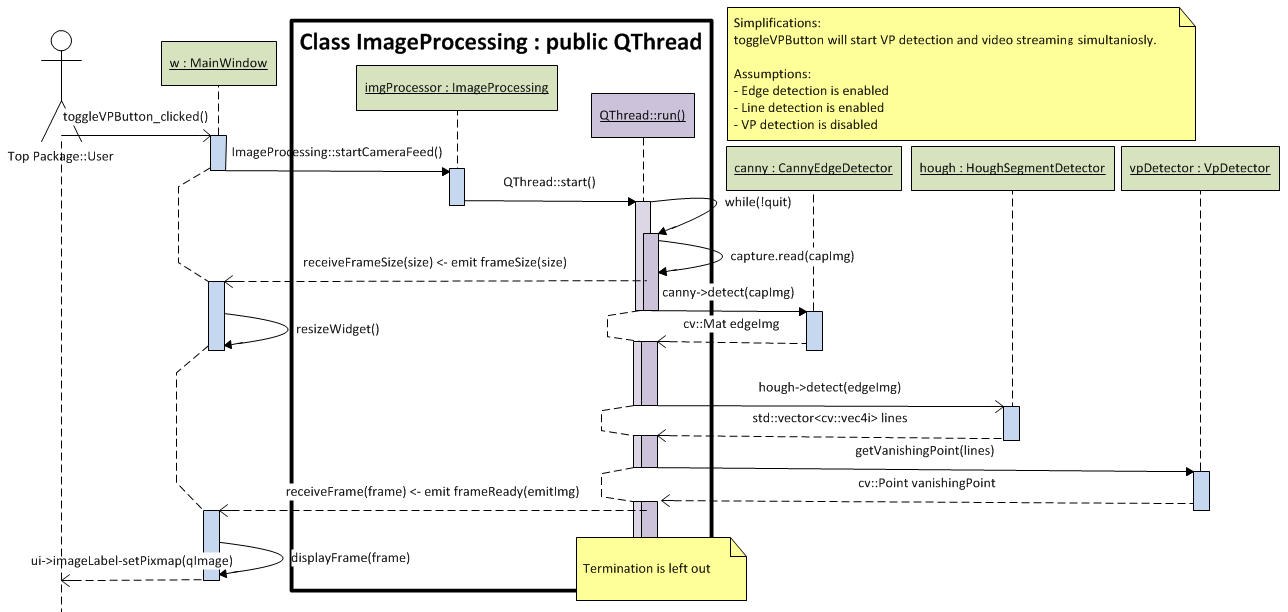
\includegraphics[scale=0.55]{VpAppSequence}
		\caption{Sequence diagram illustrating program execution when the user activates camera feed and VP detection.}
		\label{fig:VpAppSequence}
	\end{figure}
\end{landscape}



\paragraph{Graphical User Interface}

A graphical user interface was created so that the parameters for the canny edge detector and Hough lines detector could be tuned on-line. All widgets shown in figure \ref{fig:vpGui} have their functionality implemented. The user can turn on the camera feed, in this case from the web camera integrated into the laptop of the author, and switch line and edge detection on or off. Upper and lower edge detection thresholds, as well as line detection parameters can be set by using the sliders. The kernel size for the edge detector is set to 3 by 3, and can not be changed by the user. When both edge detection and line detection is enabled, the user may turn on the vanishing point detector module. In this particular application, the ellipse line filter module is not included.

\begin{figure}
	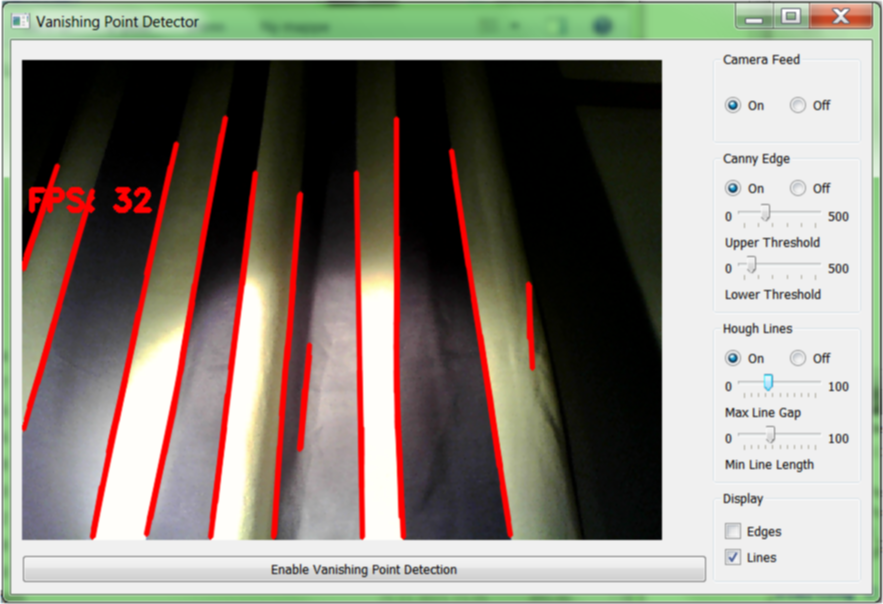
\includegraphics[scale=0.7]{VPGuiBlurred}
	\caption{Graphical user interface for the vanishing point detector. Note that the detected line segments are actually several lines overlapping each other.}
	\label{fig:vpGui}
\end{figure}

\subsection{Cause of Failure}

\section{Depth Perception and Obstruction Detection}

\subsection{Overview}

\subsection{The camera rig}

The two IP cameras were moved together to form a stereo camera. This stereo camera was used in two positions. The first camera position is on the pan-tilt module on the robot arm, see figure \ref{fig:rig_pantilt}. The second position is just over the LIDAR in front of the robot arm base, see figure \ref{fig:rig_front}.  The workshop at \gls{itk} made a mounting bracket, so that the cameras could be placed over the LIDAR. In stereo vision, it is essential that the positions of the cameras relative to each other is constant. One problem encountered throughout the project was that the camera assemby, when placed either at the pan-tilt module and over the LIDAR, was not rigid enough. The severity of this problem was somewhat alleviated by wrapping a strap around both the cameras. This camera rig is ad hoc, i.e. suitable for the purpose of this project, and a better solution should be used for succeeding projects.

\begin{figure}
	\centering
	\begin{subfigure}[b]{0.45\textwidth}
		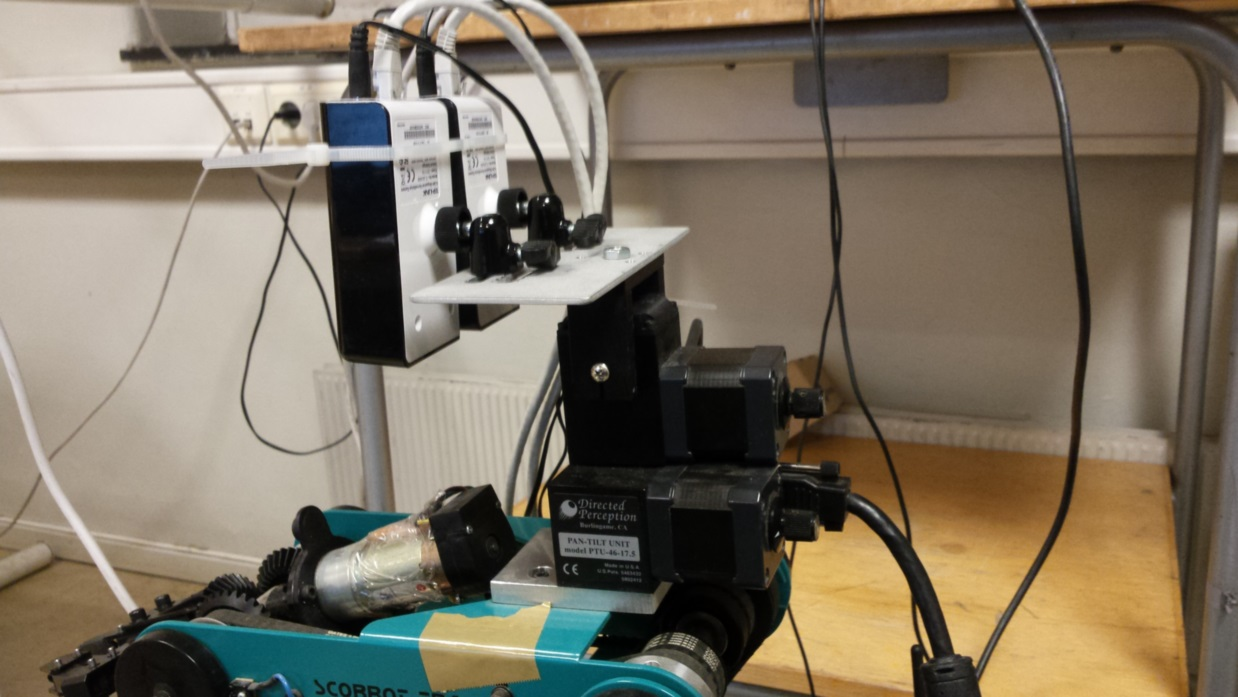
\includegraphics[width=\textwidth]{rig_pantilt}
		\caption{Camera pair mounted on the pan-tilt module.}
		\label{fig:rig_pantilt}
	\end{subfigure}
	\begin{subfigure}[b]{0.45\textwidth}
		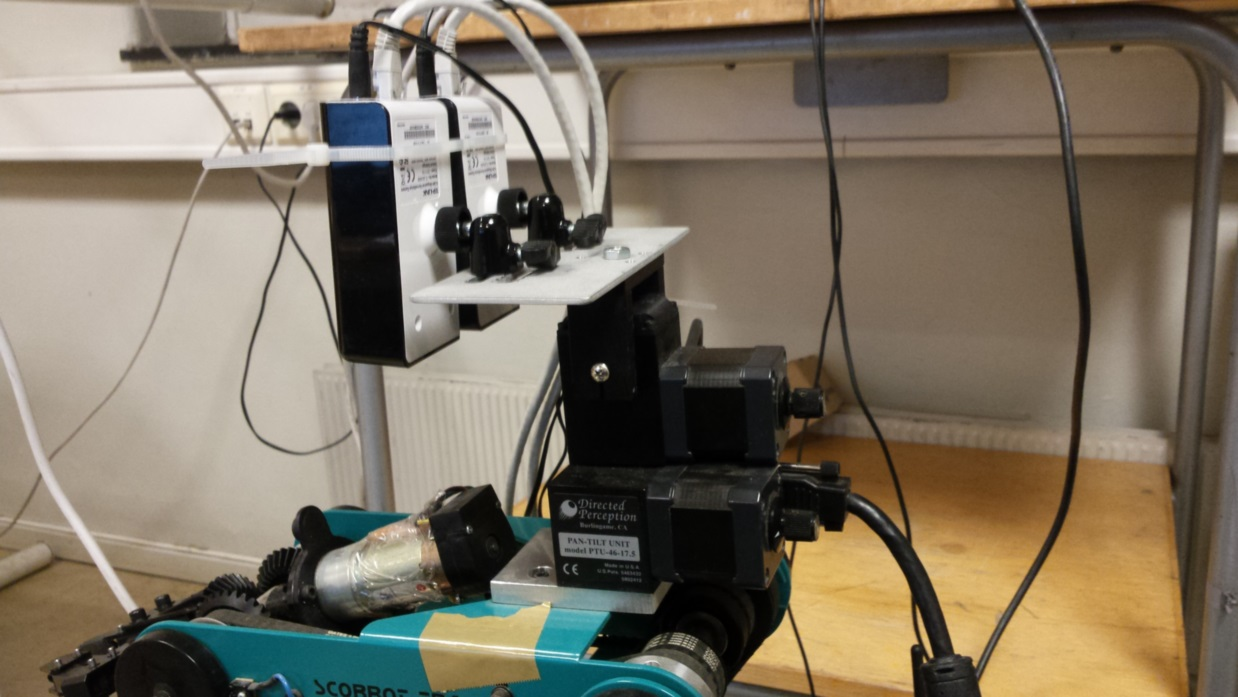
\includegraphics[width=\textwidth]{rig_pantilt}
		\caption{Camera pair mounted on the pan-tilt module.}
		\label{fig:rig_front}
	\end{subfigure}
	\caption{\label{fig:campos}The two camera positions.}
\end{figure}

\subsection{Graphical User Interface}

Tuning the parameters for stereo matching in OpenCV is a wearisome task, especially without a good graphical user interface. Figure \ref{fig:StereoGui} shows the user interface which was used to observe how parameter tuning alters the disparity map quality. Not all functionalities were implemented.

\begin{figure}
	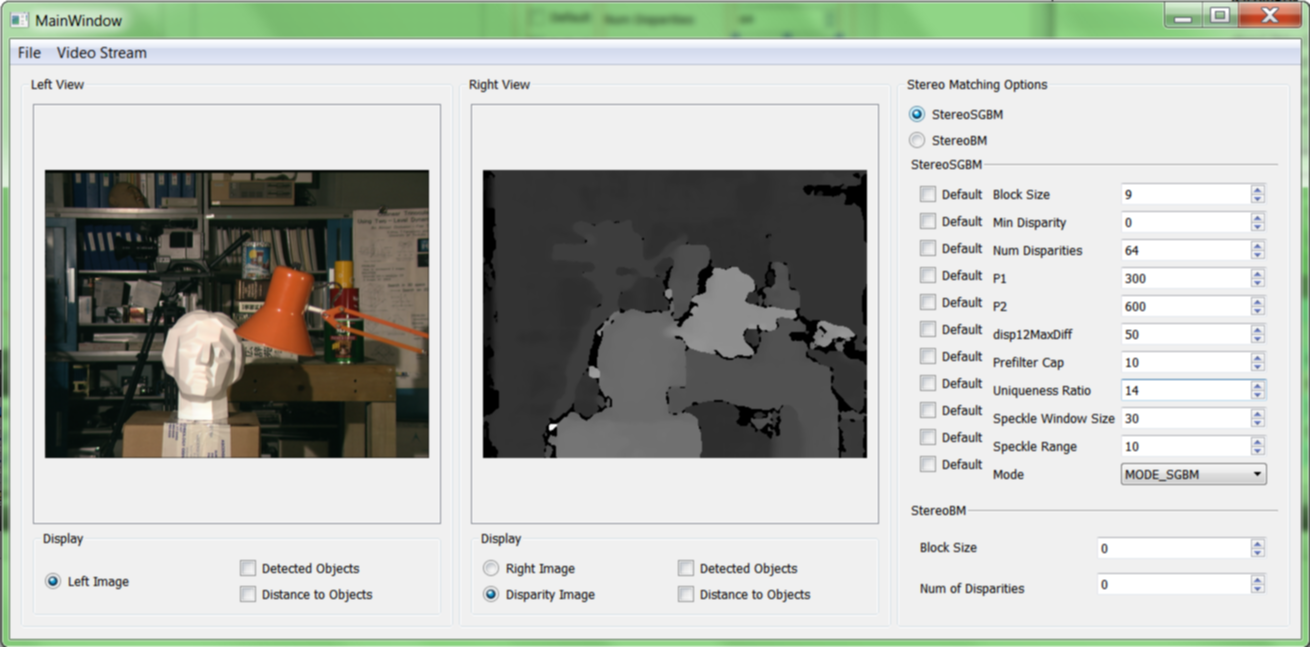
\includegraphics[scale=0.37]{StereoGui}
	\caption{Graphical user interface for stereo matching. A disparity map is computed from the Tsukuba samples by using StereoSGBM. }
	\label{fig:StereoGui}
\end{figure}

\subsection{Calibration}

As mentioned in chapter \ref{chp:theory}, all cameras will have some distortion. If the distortion is too severe, as it often will be in the context of stereo vision, the camera must be calibrated. In addition, it was assumed that the image planes were located on the same plane, and that a projection pair, for example the projections $X_L$ and $X_R$ of an object $X$, form two equal epipolar lines, $e_1$ and $e_2$, on the two image planes. In practice, these conditions are achieved through stereo calibration. The second purpose of the calibration procedure is to relate the sensor data to real world quantities, in order to measure the distance to detected objects. Code listings from Practical OpenCV by Samarth Brahmbhatt \cite{practicalopencv} has been used as a basis for calibration in this project. Some parts of his code is almost unchanged, while other parts of the listings are altered and expanded significantly. There are three steps in the calibration procedure:

\begin{enumerate}
	\item Single camera calibration.
	\item Stereo calibration.
	\item Image rectification.
\end{enumerate}

See figure \ref{fig:calibproc} for an overview of the calibration procedure. All these steps require a familiar object with known dimensions to calibrate against. Among the three calibration patterns supported by OpenCV, this implementation utilized a black and white chessboard. The chessboard has 6 by 8 squares with sides $\approx 26 \, mm$ long.

\begin{figure}
	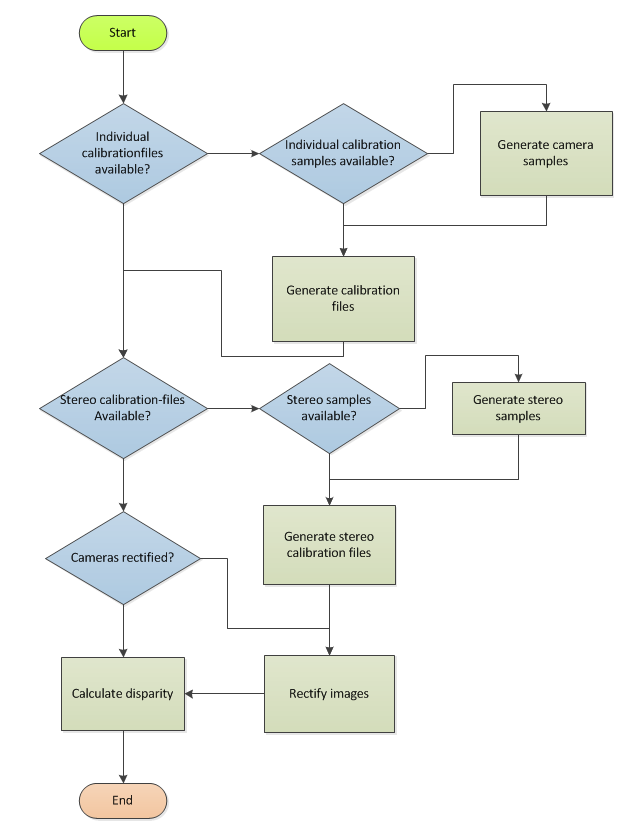
\includegraphics[scale=0.7]{StereoInit}
	\caption{An overview of the calibration procedure.}
	\label{fig:calibproc}
\end{figure}

\begin{figure}
	\centering
	\begin{subfigure}[b]{0.90\textwidth}
		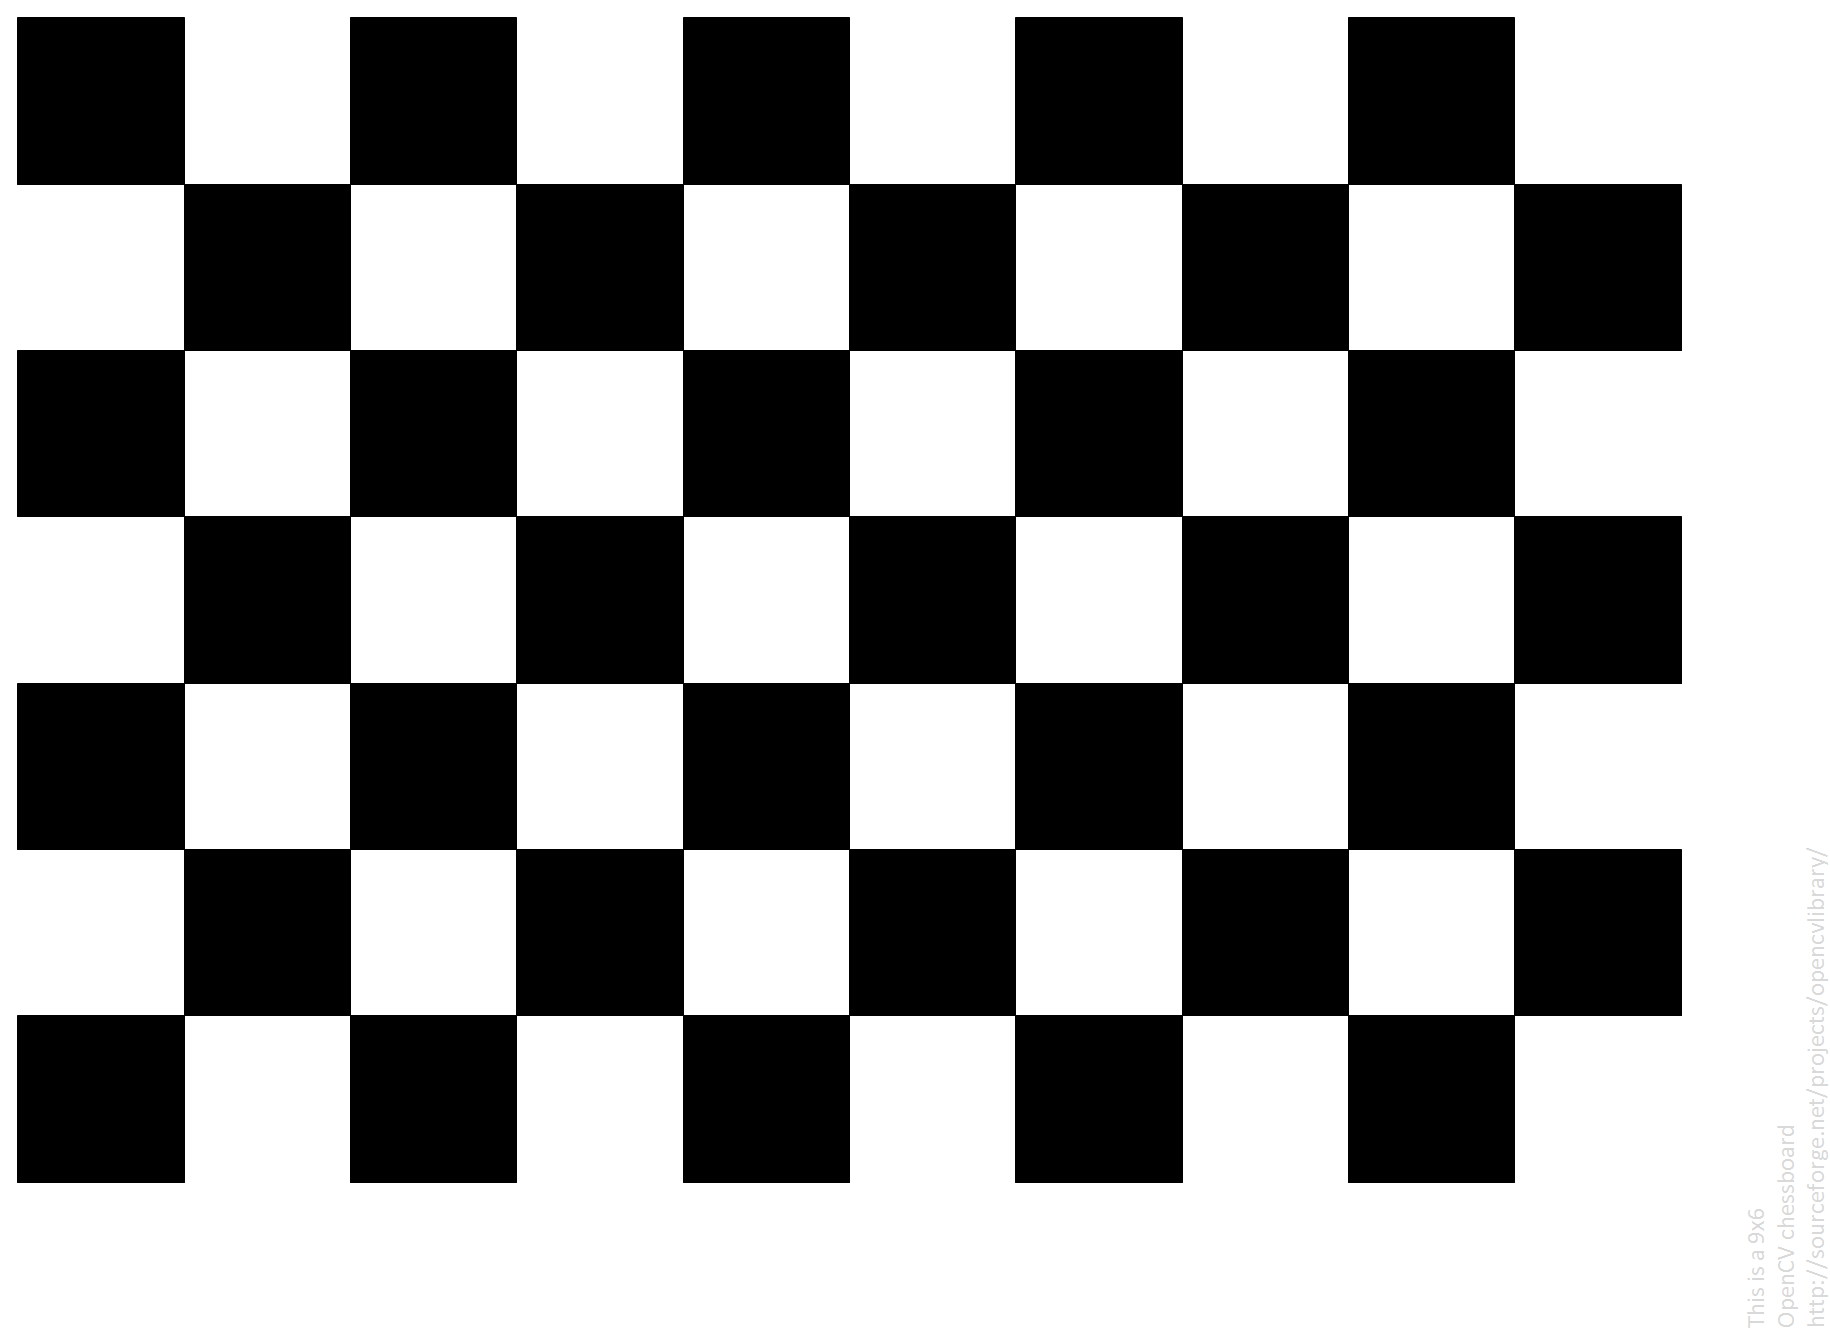
\includegraphics[width=\textwidth]{chess_pattern}
		\caption{The chessboard calibration pattern. The pattern was printed and taped to a flat surface.}
		\label{fig:chesspattern}
	\end{subfigure}
	\begin{subfigure}[b]{0.90\textwidth}
		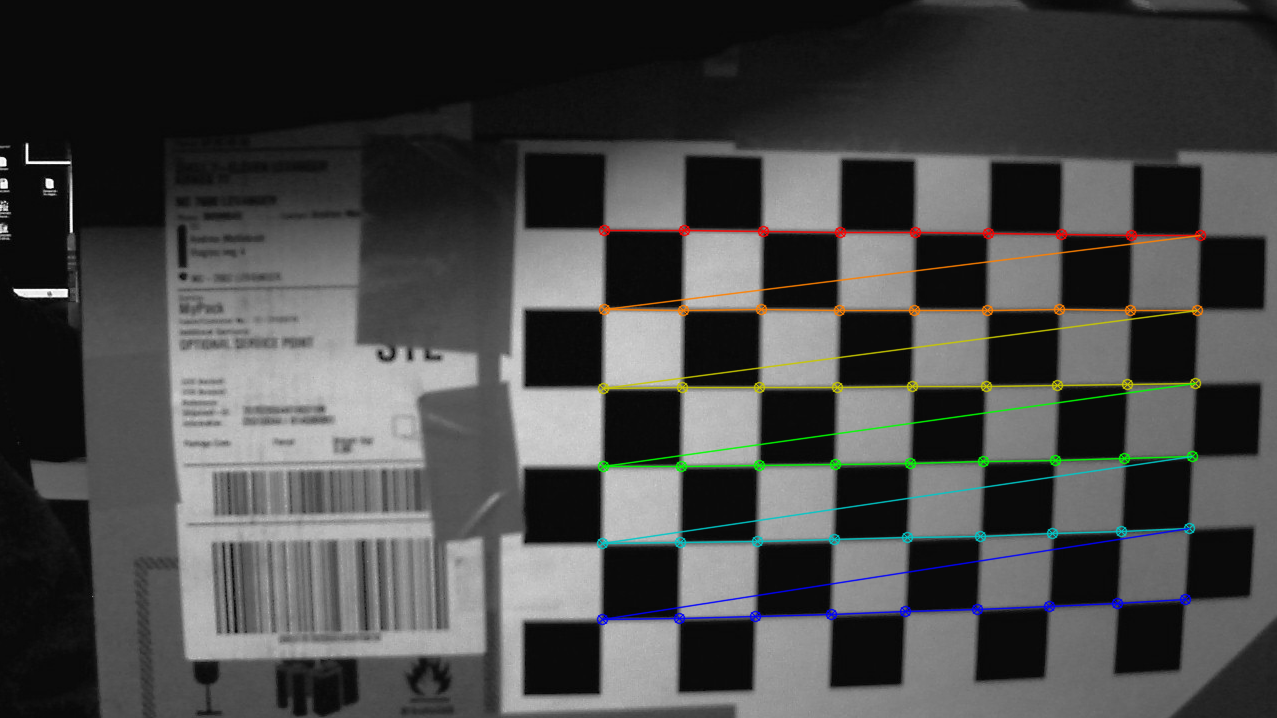
\includegraphics[width=\textwidth]{CamCalibDistorted}
		\caption{Chessboard detection. This is one of the sample images used to calibrate the camera. Note the distortion in the lower right corner.}
		\label{fig:chessdetection}
	\end{subfigure}
	\caption{\label{fig:calibrationpattern}}
\end{figure}

\paragraph{Single Camera Calibration}

In this step, the cameras are calibrated separately.  The purpose of this calibration procedure is to counter the constant radial and tangential distortion in a pinhole camera, and to relate the image pixels to real world quantities. The result of this procedure is the $3x3$ camera matrix and the five distortion coefficients mentioned in the theory chapter. The results are stored in a .xml file:

\begin{verbatim}
<?xml version="1.0"?>
<opencv_storage>
<cameraMatrix type_id="opencv-matrix">
  <rows>3</rows>
  <cols>3</cols>
  <dt>d</dt>
  <data>
    1.4478141049219482e+003 0. 6.6274484776761142e+002 
    0. 1.4432743079138295e+003 4.7609546427843065e+002 
    0. 0. 1.
  </data></cameraMatrix>
<distCoeffs type_id="opencv-matrix">
  <rows>1</rows>
  <cols>5</cols>
  <dt>d</dt>
  <data>
    -2.6128696949919589e-001 3.4600669963821584e-001
    -2.2331413545278616e-003 -2.5710895791919218e-003
    -3.7144316064113458e-001</data></distCoeffs>
</opencv_storage>
\end{verbatim}

\newpage

\begin{wrapfigure}{R}{0.4\textwidth}
\centering

	\begin{subfigure}[b]{0.35\textwidth}
        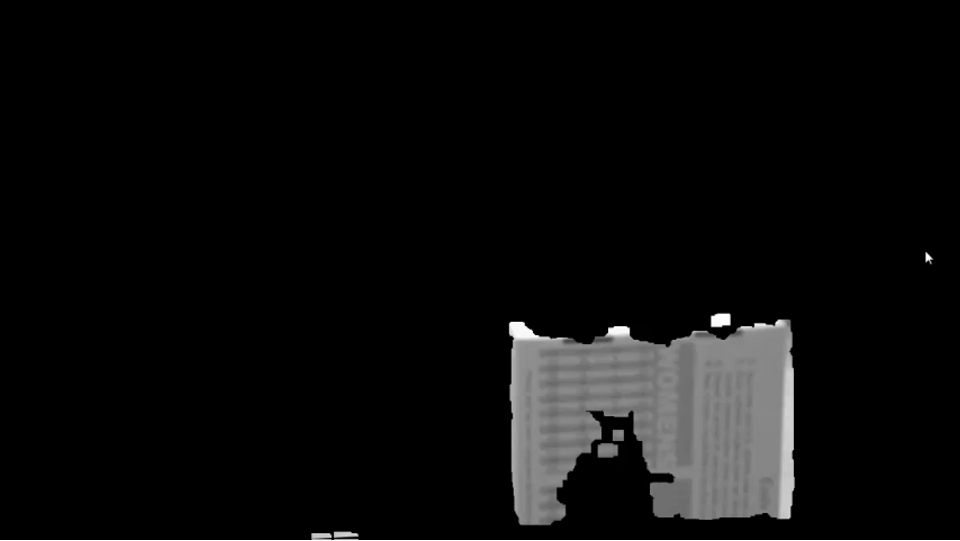
\includegraphics[width=\textwidth]{DepthLayer1}
	\end{subfigure}
	\par\medskip
	\begin{subfigure}[b]{0.35\textwidth}
        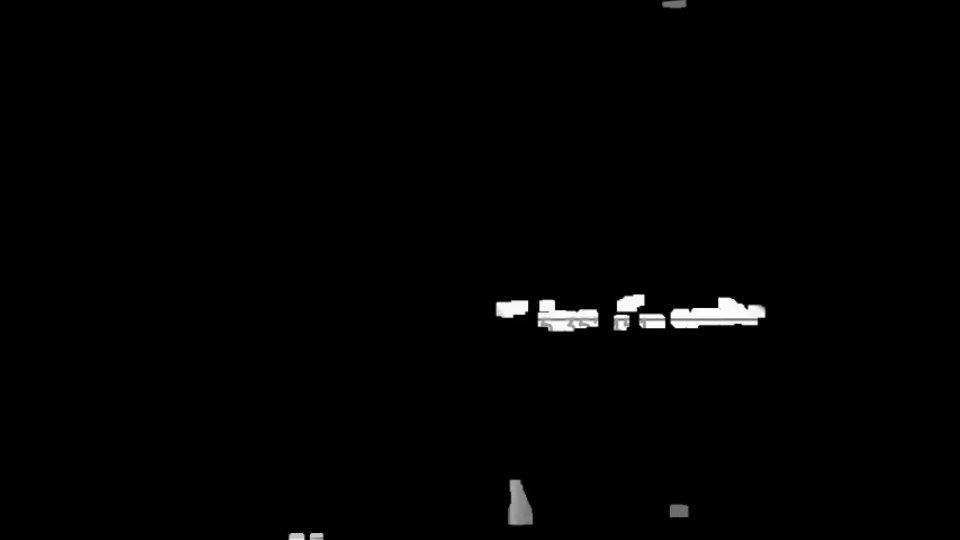
\includegraphics[width=\textwidth]{DepthLayer2}
	\end{subfigure}
	\par\medskip
	\begin{subfigure}[b]{0.35\textwidth}
        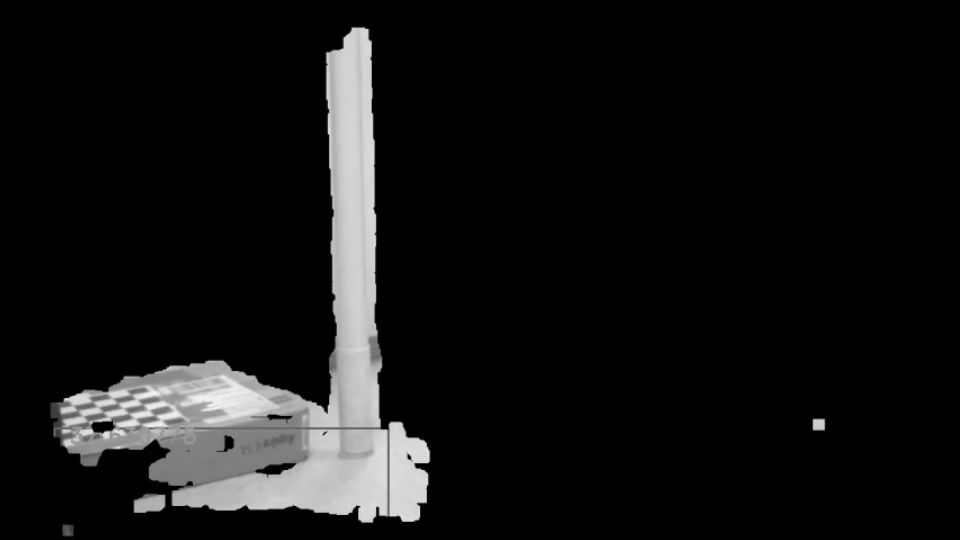
\includegraphics[width=\textwidth]{DepthLayer6}
	\end{subfigure}
	\par\medskip
	\begin{subfigure}[b]{0.35\textwidth}
        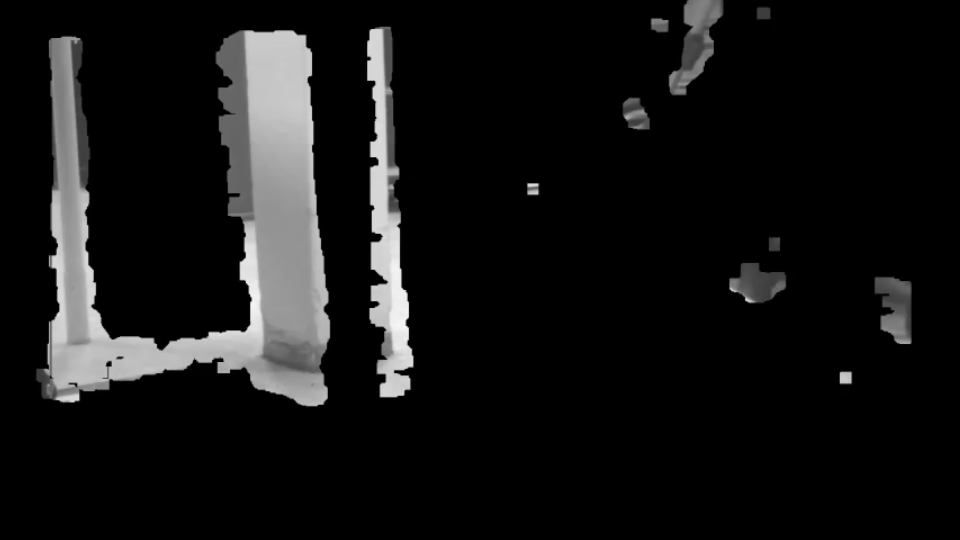
\includegraphics[width=\textwidth]{DepthLayer7}
	\end{subfigure}
	\par\medskip
	\begin{subfigure}[b]{0.35\textwidth}
        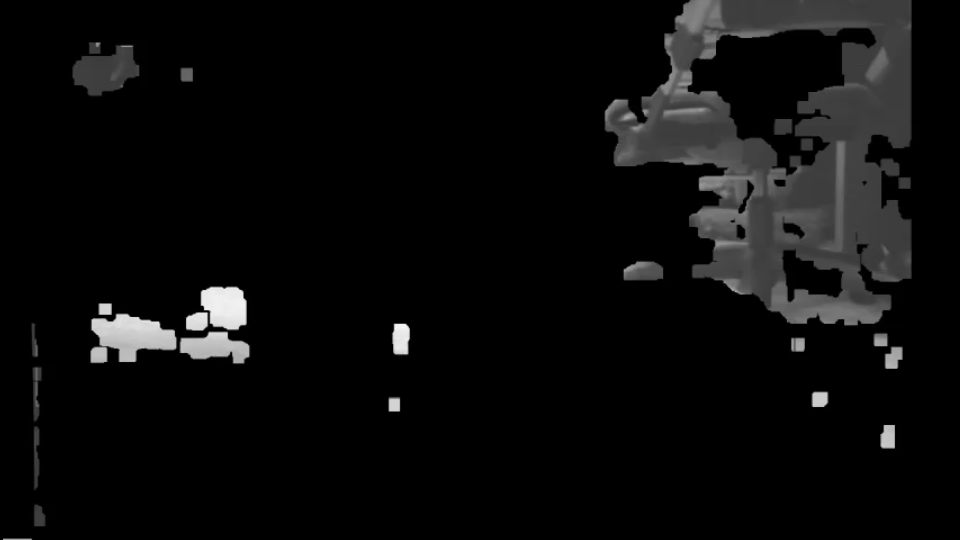
\includegraphics[width=\textwidth]{DepthLayer8}
	\end{subfigure}
	
\caption{Some of the depth layers in figure \ref{fig:StereoMatching} separated by color filtering. The top image is the closest layer, while the most distant layer is at the bottom.}
\label{fig:layers2}
\end{wrapfigure}

When all the image samples has been read into the program, the program will check if the chessboard can be detected. If the chessboard is present in the image, the position of the corners will be stored in  

\paragraph{Stereo Calibration}

\paragraph{Stereo Rectification}

%\begin{figure}
%\includegraphics[scale=•]{•}
%\end{figure}

\subsection{Stereo Matching}

\begin{figure}
\centering
 \begin{subfigure}[b]{0.45\textwidth}
        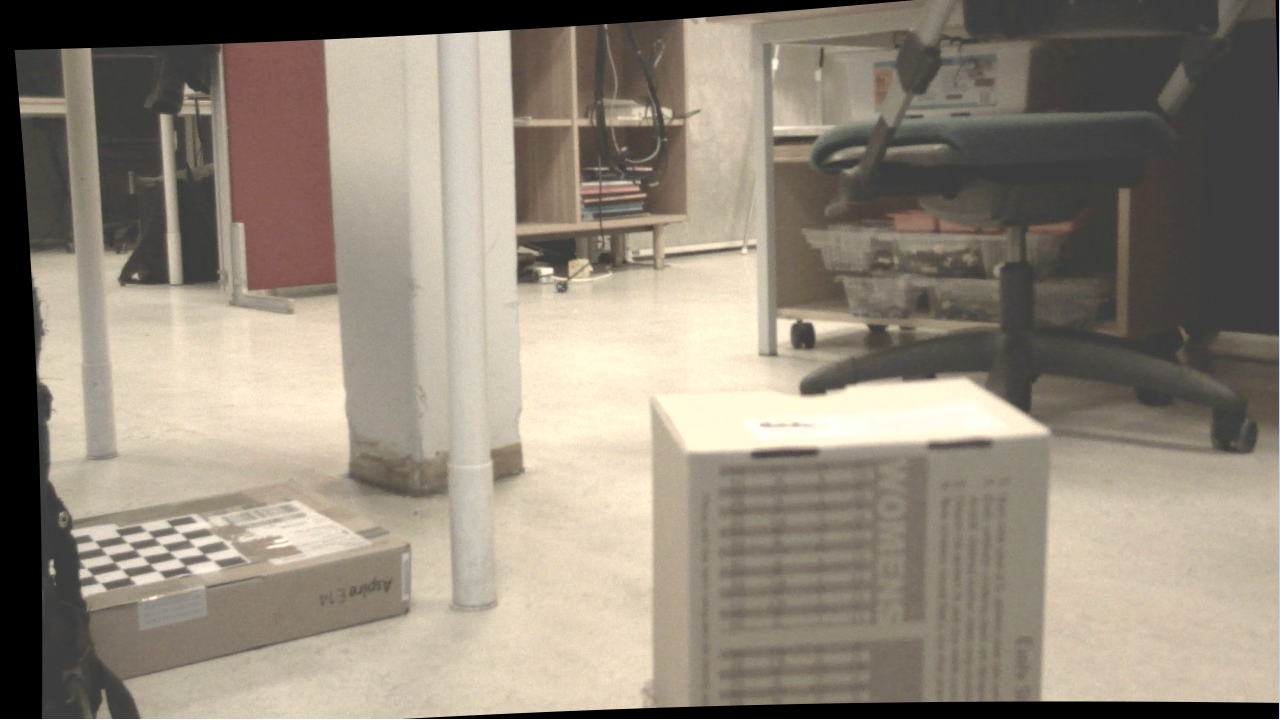
\includegraphics[width=\textwidth]{OriginalExample}
        \caption{Left camera image.}
        \label{fig:OriginalExample}
    \end{subfigure}
    \begin{subfigure}[b]{0.45\textwidth}
        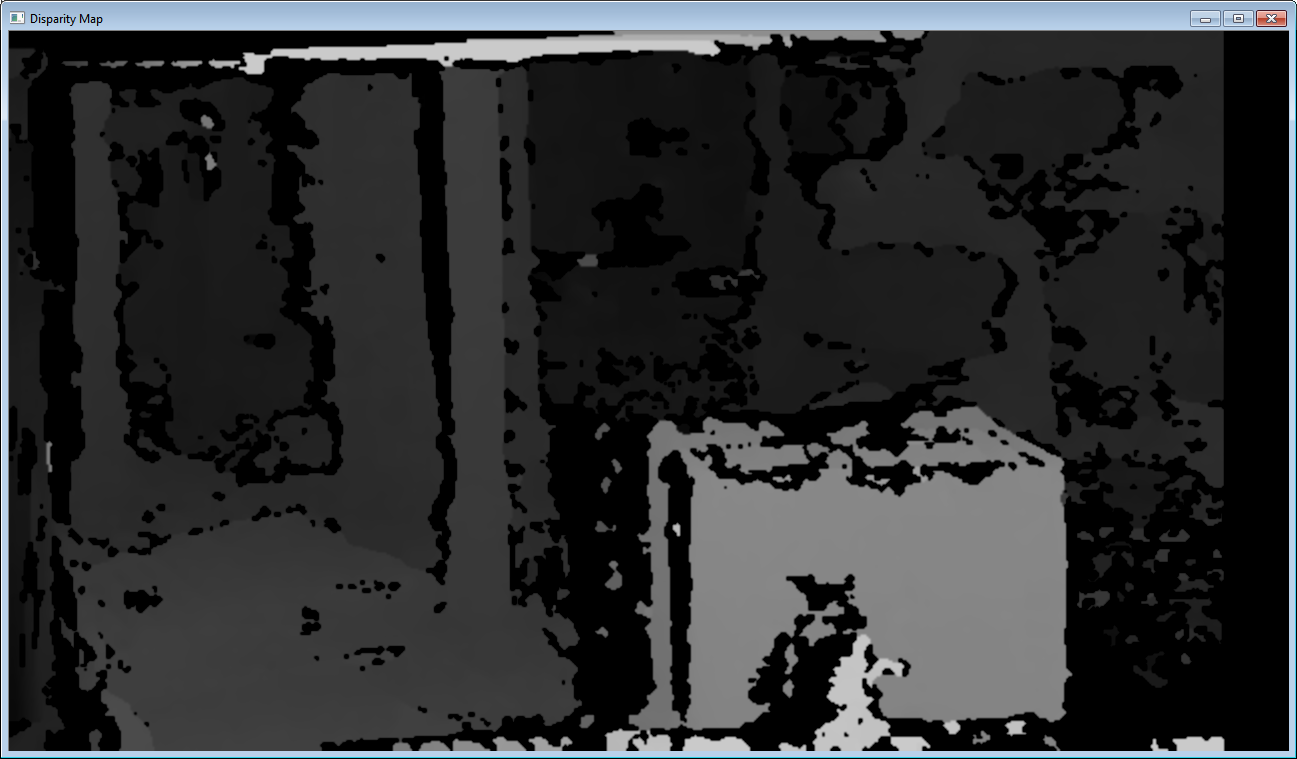
\includegraphics[width=\textwidth]{DispExample}
        \caption{Disparity map.}
        \label{fig:DispExample}
    \end{subfigure}
    \caption{\label{fig:StereoMatching}The result of StereoSGBM.}
\end{figure}

\subsection{Finding Obstructions}

\begin{figure}
	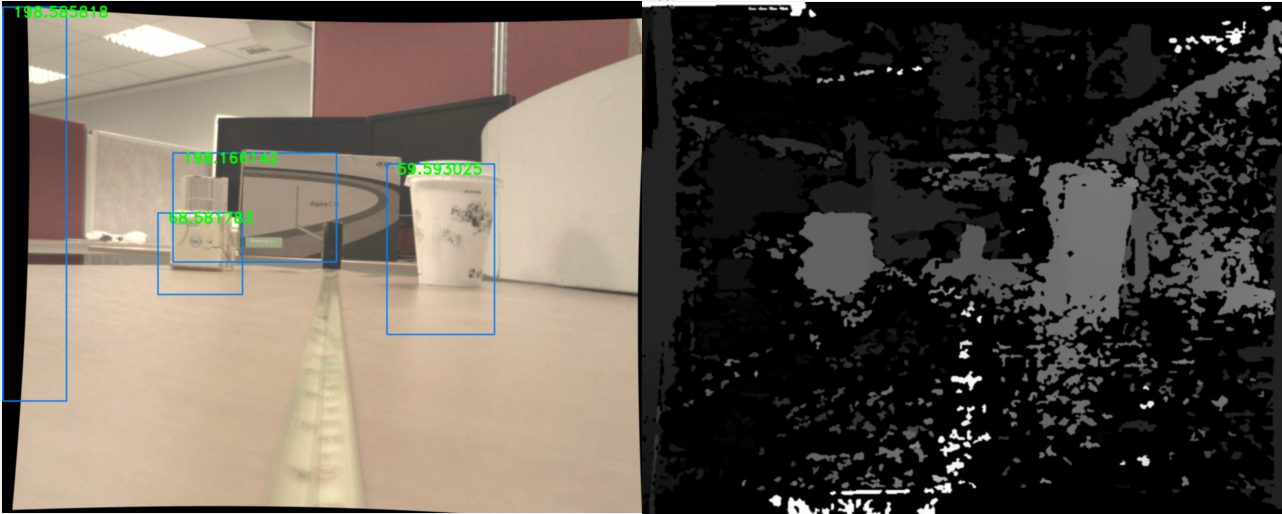
\includegraphics[scale=0.37]{obstruction}
	\caption{Dummy text. }
	\label{fig:obstruction}
\end{figure}

\subsection{Distance Measurment}

\subsection{Problems Encountered During Implementation }